\documentclass[12pt]{article}

\input preamble

\title{Principles of Parallel Architecture\\
Project Report 2}
\author{Xitong Liu \\
xliu@ece.udel.edu}

\begin{document}

\maketitle

\section{Introduction}
In this report, we will introduce the methods applied to optimize
the performance of Matrix Multiplication on parallel architecture.
Results showed that the performance has been improved a lot comparing
to the baseline approach proposed in the previous report.

\section{Baseline}
The setup of the baseline parallel is straightforward, as we divide
one matrix operand evenly into several parts, each part is distributed
to one thread. The approach is shown in Figure~\ref{fig:matrix-divide}.

\begin{figure}[h!]
	\begin{center}
		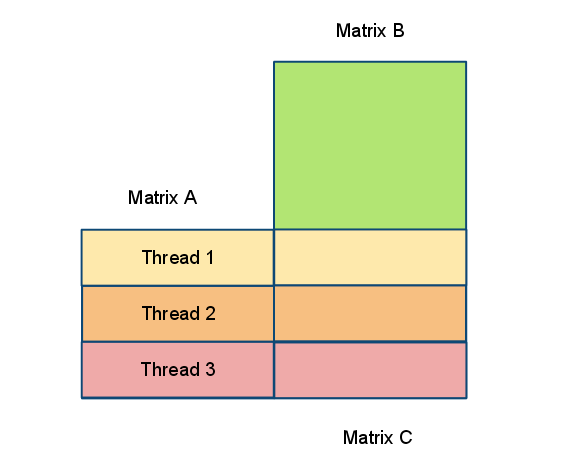
\includegraphics[width=0.5\textwidth]{matrix-divide.png}
		\caption{\label{fig:matrix-divide}Matrix Division}
	\end{center}
\end{figure}

\section{Cache Line}
In the baseline version, for $\mathbf{C}=\mathbf{A}\times\mathbf{B}$,
in the inner most loop, $\mathbf{A}$ is accessed in a row major. When 
the first element of one row in $\mathbf{A}$ is accessed, the access 
to the following elements can benefit from the cache line since they
are adjacent in memory and loaded in the same cacheline. However, 
$\mathbf{B}$ is accessed in a column major and the access of the 
following elements may cause more loads of cache line. The sample code 
for $\mathbf{C}=\mathbf{A}\times\mathbf{B}$ is shown as below:

\begin{verbatim}
DO I = 1, N 
  DO J = 1, N
	  C(I,J) = 0.0 
      DO K = 1, N
      C(I,J) = C(I,J) + A(I,K) * B(K,J) 
    ENDDO
  ENDDO
ENDDO
\end{verbatim}

We transpose $\mathbf{B}$ to $\mathbf{B^{T}}$ at first. In the 
following multiplication operation's inner most loop, access of 
both $\mathbf{A}$ and $\mathbf{B^{T}}$ is in row major and both
of them can benefit from the acceleration of cache line. More 
detail is depicted in Figure~\ref{fig:cacheline}. The sample code 
is shown as below:

\begin{verbatim}
DO I = 1, N 
  DO J = 1, N
	  C(I,J) = 0.0 
      DO K = 1, N
      C(I,J) = C(I,J) + A(I,K) * BT(J,K) 
    ENDDO
  ENDDO
ENDDO
\end{verbatim}

\begin{figure}[h!]
	\begin{center}
		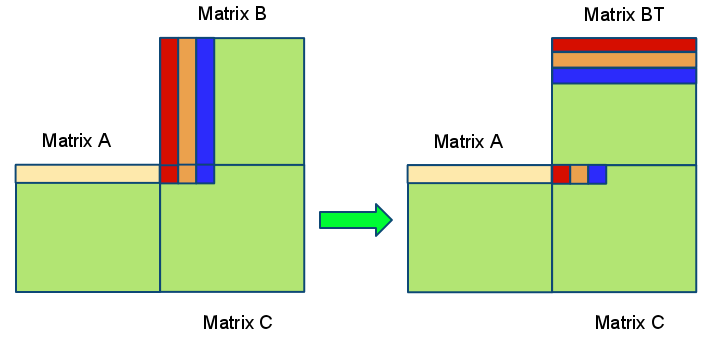
\includegraphics[width=0.7\textwidth]{cacheline.png}
		\caption{\label{fig:cacheline}Matrix Transpose}
	\end{center}
\end{figure}

\end{document}

\begin{comment}
\begin{figure}[h!]
	\begin{center}
		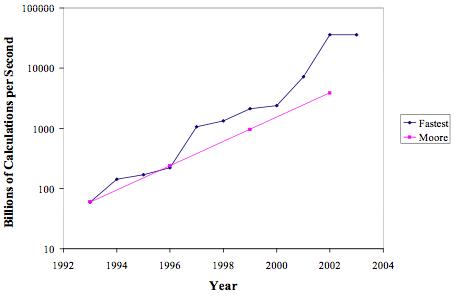
\includegraphics[width=0.7\textwidth, angle=0]{fatest.png}
		\caption{\label{fig:fatest}Fatest SuperComputer in the world}
	\end{center}
\end{figure}
\end{comment}